\chapter{Makahiki and SGSEAM Evaluation}
\label{cha:evaluation}

This chapter describes the way I evaluated the Makahiki framework described in \autoref{cha:makahiki-design} and the SGSEAM method described in \autoref{cha:sgseam-design}. First, I describe the real-world case studies of Makahiki instances realized in the Kukui Cup Challenges at the different organizations, followed by the detailed assessment of applying SGSEAM to Makahiki framework. The evaluation is to address:
(a) obtain insights about the strength and weakness of the Makahiki serious game framework, (b) obtain insights about the strength and weakness of SGSEAM serious game framework assessment method.

\section{Real-world Makahiki Instances Case Studies}

Makahiki, as a serious game framework for sustainability, has been used by different organizations to create multiple serious game instances targeting to educate and foster sustainable behavior among the communities. The first Kukui Cup Energy challenges at the University of Hawaii at Manoa (UHM) were held in 2011 for 3 weeks for over 1,000 first year students living in the residence halls. UHM subsequently held the second and third Kukui Cup Energy challenges in 2012 and 2014 for different first year students and different durations, for 9 months and 2 weeks respectively. Hawaii Pacific University (HPU) held their Kukui Cup Energy challenge in Fall 2012 and 2013 for about 200 students each year. An international organization called the East-West Center (EWC) held a Kukui Cup Energy and Water challenge for the international residents living in the residence halls. A Hawaii private school called Holy Nativity School (HNS) held a pilot Kukui Cup challenge for their elementary school students. 

\autoref{table:instances} lists these instances and their different requirements. The major differences involve the duration of the challenge, the population that could participate in the challenge, the type of resource(s) such as energy or water, whether they have smart meters installed, and the type of server hosting. Additional differences in requirements include the type of the authentication for participation and differences in game mechanics. These differences will be described in the result chapter in more detail.

\begin{table}[ht!]
  \centering
  \begin{tabular}{|p{0.12\columnwidth}|p{0.12\columnwidth}|p{0.12\columnwidth}|p{0.17\columnwidth}|p{0.07\columnwidth}|p{0.1\columnwidth}|}
    \hline
    \tabhead{Instances} &
    \tabhead{Duration} &
    \tabhead{Populations} &
    \tabhead{Resource} &
    \raggedright \tabhead{Smart meters} &
    \tabhead{Hosting} \\
    \hline
    UHM 2011 & 3 weeks & 1038 & Energy & \checkmark & Local \\
    \hline
    UHM 2012 & 9 months & 1067 & Energy & \checkmark & Cloud \\
    \hline
    UHM 2014 & 2 weeks & 1056 & Energy & \checkmark & Cloud \\
    \hline
    HPU 2012 & 3 weeks & 198 & Energy & \checkmark & Local \\
    \hline
    HPU 2013 & 3 weeks & 197 & Energy & \checkmark & Local \\
    \hline
    EWC 2012 & 2 weeks & 129 & Energy \& Water &  & Cloud \\
    \hline
    HNS 2013 & 7 months & 10 &  &  & Cloud \\
    \hline    
  \end{tabular}
  \caption{Makahiki Serious Game Instances}
  \label{table:instances}
\end{table}

The Makahiki instances deployed at these organizations have to meet these different requirements. The goal of the Makahiki framework is to minimize the effort in supporting the different requirements in various organizations. The real world case study of Makahiki is to look at the different requirements of these organizations, and how the corresponding different configurations in the Makahiki framework can be done to support these requirements, thus gain insight into how well the Makahiki framework can be used and customized in the real world scenarios. The results of the real world case studies of these instances are described in \autoref{sec:realworld-result} of the Result chapter.

\section{Applying SGSEAM to Makahiki}

This section describes a formal assessment of the strength and weakness of the Makahiki framework by applying SGSEAM to Makahiki. As described in \autoref{cha:sgseam-design}, SGSEAM is a method to assess a serious game framework based on different serious game stakeholder's experience.  
 framework in order to identified the strengths and weaknesses of both the Makahiki and SGSEAM itself.

\subsection{Step 1: Plan the Assessment}

The first step of SGSEAM process is to plan the assessment. The deliverable for this step is the assessment plan document. To complete this step, I created a tech report called ``SGSEAM Assessment Plan for Makahiki''\cite{csdl2-13-11}, also included in  \autoref{app:makahiki-assessment-plan}. The assessment plan identifies the stakeholders, determines the appropriate assessment approaches according to the available resources, choose assessment participants, and creates the assessment schedule. 

The SGSEAM assessment plan includes two categories of assessment approaches for Makahiki: the in-vivo approaches applied to the real-world UHM, HPU and EWC Makahiki instances, and the in-vitro approaches applied to the UHM ICS691 serious game course as an in-lab experiment.

 \autoref{table:assessment-plan-overview} provides an overview of assessment plan for each SGSEAM stakeholders of the Makahiki framework. \autoref{app:makahiki-assessment-plan} provides the detailed descriptions of the plan.

\begin{table}[ht!]
  \centering
  \begin{tabular}{|p{0.17\columnwidth}|p{0.34\columnwidth}|p{0.3\columnwidth}|p{0.08\columnwidth}|}
    \hline
    \tabhead{Stakeholder} &
    \tabhead{Assessment Approach} &
    \tabhead{Participants}  & 
    \tabhead{Time} \\
    \hline
    Player & Pre Post effectiveness study \newline
    	Self-reported effectiveness survey \newline
	Self-reported usability survey \newline
	Engagement metrics
	& UHM Kukui Cup players & 2011, 2012, 2014\\
    \hline
    \multirow{2}{*}{System admin} &  Post-hoc system admin interview & HPU KC sysadmin & 2012 \\
    \cline{2-4}
     & In-lab installation study & UHM ICS691 students & 2013 \\
    \hline
   \multirow{2}{*}{Game designer} & Post-hoc game designer interview & HPU \& EWC KC game designers & 2012 \\
    \cline{2-4}
     & In-lab game design study & ICS691 students & 2013 \\
    \hline
    Game manager & Post-hoc game manager interview & HPU \& EWC KC game managers & 2012 \\
    \hline
   Developer & In-lab game development study & ICS691 students & 2013\\
    \hline
  \end{tabular}
  \caption{SGSEAM Assessment Plan Overview for Makahiki}
  \label{table:assessment-plan-overview}
\end{table}

\subsection{Step 2: Gather Data}

The second step of SGSEAM process is to gather the assessment data by carrying out the assessment described in the assessment plan, recording the data and obtaining game logs. The output of this step is a data repository containing all the assessment data. 

During the period of 4 years from 2011 to 2014, the SGSEAM assessment for Makahiki was carried out by implementing different assessment approaches for the stakeholder participants, both in real-world Makahiki instances and in-lab experiments. I collected the necessary assessment data and stored them in a central location in a hard drive. \autoref{app:makahiki-data-repository} describes the content of the data repository collected from the SGSEAM assessment of Makahiki. 

The following sections describe the assessments and the data collected. 

\subsubsection{Player Assessment}

We used the real-world Makahiki instances at the University of Hawaii at Manoa to assess the players' experience with Makahiki. 

To assess the effectiveness of the framework for designing games that improve player literacy in sustainability, we
conducted two energy literacy surveys, one before the challenge (pre-game) and one after
the challenge (post-game). SurveyGizmo was used to create the surveys which consists of the set of sustainability literacy and behavior questionnaires. 
After the surveys were completed, the responses saved in SurveyGizmo were exported to be stored in the SGSEAM assessment data repository.

To assess the effectiveness of the framework for designing games that produce positive change in sustainability
behaviors, we recorded and analyzed energy consumption data before, during and after the
challenge, and stored the energy consumption data into the SGEEAM assessment data repository. 

We also conducted the in-game self-reported behavior changes survey. The survey asked questions about player interests in sustainability prior to and after the game, as well as any perceived behavior changes when playing the game.  To assess the usability of the game produced by the Makahiki framework, we conducted an in-game usability survey. The survey asked questions about the players' experience with respect to the user interface of the game. The surveys were administered using SurveyGizmo service. The responses were exported to be stored in the SGSEAM data repository.

In addition to the surveys and energy data, we collected the game and log data to calculate the engagement metrics to assess the engagement level of the instance. The game data which were saved in the Makahiki database were exported and stored in the SGSEAM data repository.

The following lists the data collected with regarding to the SGSEAM player assessment:

\begin{itemize}
\item Pre-post surveys from players;
\item Energy data before, during, and after the game; 
\item In-game survey from players;
\item Game data and logs (participation and submissions)
\end{itemize}

\autoref{app:makahiki-data-repository} describes the content of these data in the data repository.

\subsubsection{System Admin Assessment}

There are two approaches described in SGSEAM plan to assess the system admin's experience: One is the interview of the system admin of a real world instance, the other is the in-lab experiment with ICS691 serious game development class.

In order to gain insights on the experience of a real world system admin who uses the Makahiki, I performed interviews with the system admin of the Hawaii Pacific University (HPU) challenge.  I also collected the email exchanges with the system admin regarding the installation process and maintenance of Makahiki system. Both interview audio recordings and email exchange data were stored in the SGSEAM data repository.

In the in-lab experiment, the students in the ICS691 Spring 2013 class were tasked with installing the Makahiki system into their local computers as well as the cloud environment. In order to understand how much time it takes to install the Makahiki and what problems might be encountered, a Google form were used to describe the steps for installing Makahiki both locally and in the cloud. For each step, Students were asked to record the time they spent and the problems they encountered. \autoref{app:googleform} includes the complete installation Google form used for Makahiki system admin assessment.

The students were also asked to provide feedback about their installation experiences in the form of blog posts. The responses from the Google form and the blog posts were exported and stored in the SGSEAM data repository.

The following lists the data collected with regarding to the SGSEAM system admin assessment:

\begin{itemize}
\item Interview audio recordings with system admins;
\item Email communications with system admins;
\item Google form responses from ICS691 installation experiment; 
\item Blog posts from ICS691 installation experiment
\end{itemize}

\autoref{app:makahiki-data-repository} describes the content of these data in the data repository.

\subsubsection{Game Designer Assessment}

Similar to the SGSEAM system admin assessment, there are also two approaches described in SGSEAM plan to assess the game designer's experience: interview and in-lab experiment.

I performed the interviews with the real-world game designers of the Hawaii Pacific University challenge and the East West Center challenge. I asked them about their game designing experiences using the Makahiki game design admin interface. The email exchanges with the game designers regarding the game design process were also collected. Both interview audio recordings and email exchange data were stored in the SGSEAM data repository.
 
The students in the in-lab experiment were tasked to design a Kukui Cup-like serious game using Makahiki. I designed another Google form to ask students to follow the designing steps and record their time and problems encountered during their designing process. \autoref{app:googleform} has the complete game design Google form for the steps the students need to follow. The students were also asked to provide feedback about their installation experiences in the form of blog posts that discussed the difficulties and problems they encountered during the game design process.

The data collected from the Google form response and the blog post from the students was analyzed. The results are described in \autoref{sec:designer-in-lab-result} of the Results chapter.

The responses from the Google form and the blog posts were exported and stored in the SGSEAM data repository.

The following lists the data collected with regarding to the SGSEAM game designer assessment:

\begin{itemize}
\item Interview audio recordings with game designers;
\item Email communications with game designers;
\item Google form responses from ICS691 game design experiment; 
\item Blog posts from ICS691 game design experiment
\end{itemize}

\autoref{app:makahiki-data-repository} describes the content of these data in the data repository.

\subsubsection{Game Manager Assessment}

I performed the interviews with the game managers of the Hawaii Pacific University challenge and the East West Center challenge to study the experience of game management using Makahiki. I also collected the email exchanges with the game managers regarding the game management process. Both interview audio recordings and email exchange data were stored in the SGSEAM data repository.

The following lists the data collected with regarding to the SGSEAM game designer assessment:

\begin{itemize}
\item Interview audio recordings with game managers;
\item Email communications with game managers;
\end{itemize}

\autoref{app:makahiki-data-repository} describes the content of these data in the data repository.

\subsubsection{Developer Assessment}

I performed the in-lab game development experiment with the students participating in the ICS691 serious game development class. The students in the experiment were tasked with developing an enhancement to the Makahiki instance. This involved setting up the development environment, following the tutorial to create the ``Hello world'' widget using Makahiki, and finally, developing an enhancement which extends the functionality of the Makahiki system. 
The students were asked to submit their development source code to the public source code repository (Github) and write a blog post to discuss their efforts to complete the development activity.

The blog posts were exported and stored in the SGSEAM data repository. The following lists the data collected with regarding to the SGSEAM game designer assessment:

\begin{itemize}
\item Blog posts from ICS691 game design experiment
\end{itemize}

\subsection{Step 3: Produce Assessment Report}

After the assessment approaches were carried out and data collected, the data was analyzed to determine the strengths and weaknesses of the Makahiki framework. The results of the analysis are described in the \autoref{sec:assessment-result} of the following Results chapter. The final deliverable of the SGSEAM assessment process was created as the improvement action report described in \autoref{app:makahiki-improvement-report}.

\section{Consent from Human Research Study Subjects}
This research interviewed and studied the behaviors of several human subjects including:

\begin{itemize}
\item First year students who played the real world UHM Kukui Cup instances for 2011, 2012 and 2014
\item Students who participated in the UHM ICS691 in-lab experiment study
\item Administrators who used Makahiki to install, design, and manage the real world Kukui Cup instances in HPU and EWC
\end{itemize}

We had obtained their consent to participate into this research from all the above human subjects. The study is also approved by Office of Research Compliance at the University of Hawaii Human Studies Program under the CHS \#20451.

\section{SGSEAM Assessment plan for Lucid BuildingOS}

With the hope to collaborate with Lucid Design Group to apply SGSEAM to their Building OS and Building Dashboard serious game framework, I created the SGSEAM assessment plan for them. The plan is described in \autoref{app:sgseam-lucid-guide} as part of the proposed SGSEAM assessment guide for Lucid BuildingOS. 

\autoref{table:lucid-approaches} shows the approaches we recommended
for each stakeholder in the case of Lucid BuildingOS framework.
 
\begin{table}[ht!]
  \center
  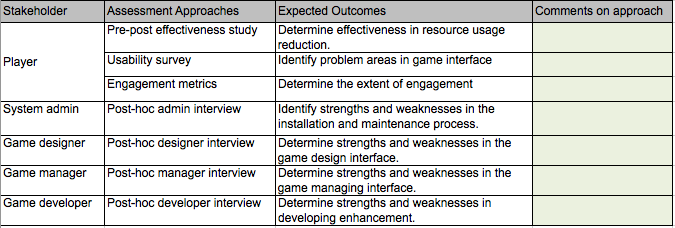
\includegraphics[width=0.95\columnwidth]{approach}
  \caption{BuildingOS Assessment Approaches}
  \label{table:lucid-approaches}
\end{table}

Comparing to the approaches of the SGSEAM assessment of Makahiki, the recommendation mainly consists of {\em in-vivo} approaches, such as post-hoc interviews, pre-post test, and in-game surveys. While an in-lab experiment such as the one done in Makahiki is more rigorous, we believe it is too expensive for Lucid's assessment. On the other hand, the in-vivo data reflect the real world interaction between the stakeholders and the framework, thus providing better insight in the real world settings.

By carrying out the assessment described in the plan, we hope to identify the major strengths and weaknesses of the Lucid's BuildingOS framework from the perspectives of major stakeholders, and provide recommendations to any actionable improvements to the developers of the framework.

\section{Limitations}

There are several limitations to this evaluation design. SGSEAM is designed to assess any serious game framework from the five major serious game stakeholder's perspectives. We only apply SGSEAM to one serious game framework, Makahiki, which is also designed by us. I have biases resulting from my experience implementing Makahiki that may affect the design of the SGSEAM, as a result of which some of the assessment approaches might not be effective in assessing other serious game framework. As described in \autoref{future:other-framework} of the ``Future Directions'' section, BuildingOS\cite{building-dashboard} by Lucid Design Group, another serious game framework, is a good candidate to be applied with SGSEAM. Our research lab made an effort to contact Lucid Design group for the collaboration. I created the assessment plan (\autoref{app:sgseam-lucid-guide}) for them which we hoped would lead to the application of SGSEAM to the BuildingOS system. But due to the workload of the Lucid design group, the collaboration did not continue.

Without another data point of the application of SGSEAM, there is not enough confidence in the evaluation of the SGSEAM itself. 

One limitation in the application of SGSEAM to Makahiki is the small sample size in the post-hoc interview approach. Due to the nature of the this kind of serious game, it is common to have just one or two system admin(s), game designer(s), and game managers(s). It is often the case that the game designers are the same as the game managers. In our evaluation design, although there are 7 Makahiki game instances in 4 organizations, we can only interview 1 system admin from HPU instance, 3 game designers who is also game managers from HPU and EWC instances. The UHM instances were designed and managed by ourself. We also installed and deployed the instances except the HPU ones, so there is no other sys admin candidate.  

Although the in-lab experiment study is a good approach to overcome the small sample size limit of the post-hoc interview approach, the ICS691 students participating in the system admin experiment might not reflect the typical system admin population because of the different skill set, thus limited the accuracy of the assessment results. On the other hand, it would be difficult or expensive to choose a group of participants with system admin skills.

Given this limitations, the application of SGSEAM to Makahiki still resulted in useful insights into the strengths and weaknesses of the Makahiki framework.

\section{Summary}

This chapter described the evaluation design for both Makahiki and SGSEAM.  Makahiki, as a serious game framework for sustainability, has been used by different organizations to create multiple serious game instances targeting education and fostering of sustainable behavior among the communities. The real world case study of Makahiki is to look at the different requirements of these organizations, and the corresponding different configurations in the Makahiki framework to support such requirements. A more formal assessment of the strength and weakness of the Makahiki framework is to apply SGSEAM to Makahiki.

Following the SGSEAM process, the assessment plan (\autoref{app:makahiki-assessment-plan}) was created as the first deliverable of the process, also as a techical report \cite{csdl2-13-11} to guide the SGSEAM assessment of Makahiki. The assessment plan identifies the participants in the categories of five SGSEAM stakeholders. Two categories of assessment approaches were determined. The {\em in-vivo} assessment approaches of pre-post effectiveness study, in-game surveys and post-hoc interviews were applied to the real-world Kukui Cup challenges created by the Makahiki framework, to assess the experiences of players, system admins, game designers, and game managers. The {\em in-vitro} assessment approaches of in-lab study used the UHM ICS691 serious game course to assess the experiences in game installation, game design and game development. The assessment schedule was also created during the planning step.

After creating the assessment plan, I carried out the Makahiki assessment according to the SGSEAM plan, a data repository (\autoref{app:makahiki-data-repository}) was created to collect all the assessment data. The data was analyzed to determine the strengths and weaknesses of the Makahiki framework. The results of the analysis are described in the \autoref{sec:assessment-result} of the Results chapter. The final deliverable of the SGSEAM assessment process was created as the improvement action report described in \autoref{app:makahiki-improvement-report}.
